\chapter{Granularity of Specificationss}
\label{chap:granularity}
The specification of requirements is an important part the development of critical systems, and the analysis results are greatly dependent upon these specifications. Formal specification, as described in Section~\ref{sec:formalSpec}, is the translation of the informal system requirements into a mathematical logic to determine if the system design is correct~\cite{hinchey2012industrial}. The informal system requirements are often initially developed and written in natural language which is often ambiguous and always mathematically informal. The formal semantics of specified properties, such as LTL, is fully defined and thus is tractable to mathematical reasoning; this does not imply that formalization is fool-proof or straightforward to do~\cite{kotonya1998requirements}. 

 In the approach of system development and safety assessment of models that we describe in this research, we define these specifications in the form of \emph{guarantees} of the behavior of components and \emph{assumptions} regarding the environment. The verification task is to show that a system guarantee $P_s$ is provable given the behavior of its subcomponents $C_s$ and the system assumption $A_s$. A systems engineer must translate natural language requirements into these formal contracts for each component. If there are dependencies between contracts or irrelevant subexpressions within the statements, this may change the analysis results. 
 
The reason this is of interest to us is due to the use of MIVCs in the generation of minimal cut sets. Previous work has shown that the specification and formulation of the guarantees can affect the IVC analysis results~\cite{ghassabani_2018}. The algorithm used to generate the cut sets based on MIVC results may lead to the loss of minimality with regard to the cut set.  Assume that there is a single critical guarantee $g$ that is required to prove a safety property. This will be in the MIVC generation and the associated fault activation literal will be in the cut set. Assume the structure of the guarantee is $g = A \land B$ for Boolean formulae $A$ and $B$. There are also two leaf level faults, one that affects the truth value of $A$ and one that affects $B$. Of course either will violate the guarantee -- and hence be in the cut set, but if only $A$ is needed for the proof of the property, there will be more faults in the cut set than minimality suggests. 

To address this problem, we begin the exploration of granularity and automated methods to solve this problem. This chapter outlines our exploration into this topic. 

\section{Background Research and Foundation}
As described in Chapter~\ref{chap:prelim}, a transition relation is considered to be a conjunction of Boolean formulas. Depending on how contracts are specified in the model, it is possible to have a ``complete" specification, i.e., all of the equations in the model are required to determine the validity of the property. However, in certain cases, subexpressions of equations may be irrelevant. If the equation is decomposed into smaller pieces, this incompleteness becomes visible and the model is no longer completely {\em covered}. Simply put, coverage is a metric that determines how well properties cover the design of a model. It is often the case that splitting an equation of the model into more conjuncts, or equivalently, making the model more \textit{granular}, leads to lower coverage of the model. 

This can be seen in the IVCs generated for a given safety property. The intuition can be illustrated with a small example. If the safety property is: $P : A $ for some complex formula $A$ and an equation in the model is $g: A \land (B \lor C)$, the supporting equation $g$ will be an IVC. But $g$ also contains other statements that do not necessarily support the proof of $P$ -- the only portion of $g$ that matters to the proof is $A$. The IVCs in a more granular model would theoretically reflect only the necessary equations required for property verification, and thus would provide more specific analysis results. A more granular model in this small example could be $g_1 : A$ and $g_2: B \lor C$. Then we would see only $g_1$ in the IVC elements for $P$. 

Interestingly, similar work from a varied perspective has been done in test case generation, specifically \emph{Modified Condition and Decision Coverage} (MC/DC). It was found that MC/DC over implementations with structurally complex Boolean expressions are generally larger and more effective than MC/DC over functionally equivalent but structurally simpler implementations~\cite{gay2016effect}. An automated technique called \emph{inlining} provides a restructuring of the model by inlining simpler Boolean expressions into a single, now more complex, expression. An example of an unlined implementation is: 

\begin{figure}[h]
	\begin{center}
		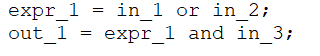
\includegraphics[scale=1.0]{images/uninlinedEx.PNG}
	\end{center}
	\vspace{-1.5em}
	%\caption{Uninlined implementation example}
	%\label{fig:uninlined}
\end{figure}

And the associated inlined implementation is: 

\begin{figure}[h]
	\begin{center}
		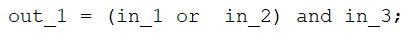
\includegraphics[scale=1.0]{images/inlined.PNG}
	\end{center}
	\vspace{-1.5em}
	%%\caption{Inlined implementation example}
%	\label{fig:inlined}
\end{figure}

Inlining results in a behaviorally equivalent implementation with different structure (syntax). The reason MC/DC provides much greater coverage in terms of test case generation is because MC/DC on an inlined system will require specific combinations of input that will not be required to achieve coverage of the noninlined system~\cite{gay2016effect}. 

Inductive validity cores, on the other hand, attempt to answer a different kind of question about the model than test coverage. In the IVC case, the goal is to find the minimal sets of model elements that contribute to a proof of a safety property. When these model elements are pulled from the model in terms of guarantees and assumptions, the \emph{granularity} of these logical statements matters in the opposite way. The IVC algorithm performs no deeper traces than those defined in those model elements (guarantees/assumptions). For our purposes, it is beneficial at times to see which \emph{parts} of the contract are necessary for the proof. In this case, instead of making the contracts more complex (inlining), we wish to simplify the contracts (un-inlining). In this way, the IVCs are more specific with regard to which parts of the contract are vital to the proof. This will theoretically decompose the contracts and eliminate property dependencies within the model. 

Granularity of contracts for IVCs has been briefly discussed by Ghassabani~\cite{ghassabani_2018}, but to our knowledge has not been discussed in any other previous work -- in particular related to minimal cut set generation. Since IVC generation is a required first step of our minimal cut set algorithms, it is important to discuss how the granularity of the model will affect the cut sets generated through this approach. 

As described in Chapter~\ref{chap:mcsGen}, the backend model checker used in this transformation is \jkind which performs $k$-induction over a transition system defined with a Lustre program. Ghassabani performed a preliminary investigation of granularity within the context of the Lustre language. Lustre provides an adequate formalism for this discussion because it is top-level conjunctive, equational, and \textit{referentially transparent}~\cite{Halbwachs91:IEEE}. This means that the behavior of a Lustre program is defined by a system of equations and any subexpression on the right side of an equation can be extracted and assigned a fresh variable\footnote{A fresh variable is a variable with an identifier that has not been used within the program.} which is substituted into the original equation without changing the meaning of the program. In this context, \textit{granular refinement} is defined as an extraction of a subexpression into a new equation assigning a fresh variable. 


\section{Illustrative Example Showing the Effects of Granularity}
To see how different representations of the system will alter the IVC and MinCutSet computations, let us examine a simple sensor example system. In this simple AADL architecture, the environmental temperature and pressure is sent to a subsystem of sensors which contains a temp sensor and a pressure sensor, both of which receive the respective environmental inputs. If the temperature (or pressure) surpasses a given threshold, then the temp (pressure) sensor outputs a HIGH\_LEVELS flag. It also outputs the temperature (pressure) reading seen at the sensor. A diagram showing the two levels of the AADL implementation is shown in Figure~\ref{fig:sensorGran1}.  

\begin{figure}[h]
\begin{center}
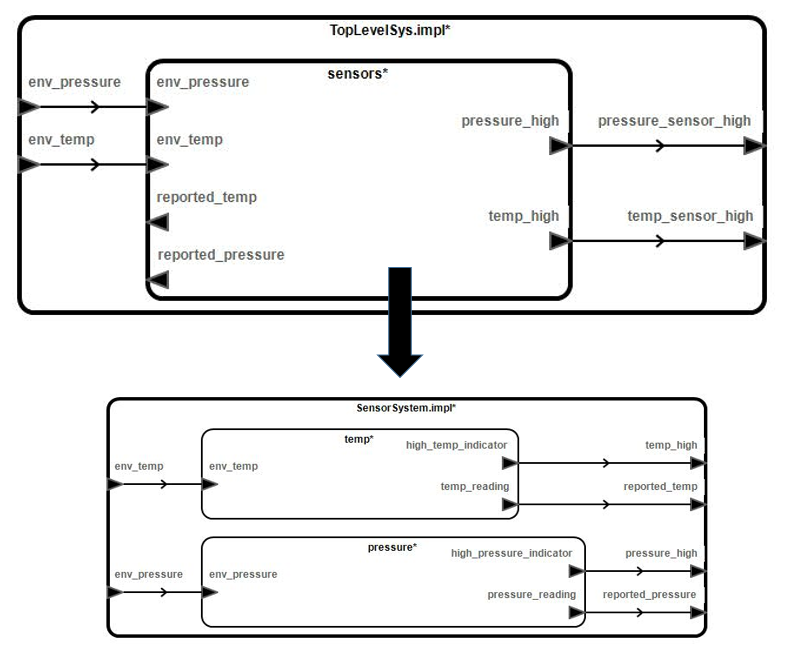
\includegraphics[width=14cm]{images/sensorGran.png}
\caption{Tempurature Sensor System} 
\label{fig:sensorGran1}
\end{center}
\end{figure}

Now that the basic architecture is in place, we focus our attention on the requirements of each component. The behavior we wish to enforce at the temperature sensor level corresponds to the following two guarantees, $G_1$ and $G_2$. (Note: pressure sensor behavior is quite similar and for this reason, we will stick to the temperature for this example.) 

$G_1$: If environmental temperature surpasses threshold, then output high temperature indication: \textit{(temp $>$ THRESHOLD) $\implies$ (high\_temp\_indicator)}

$G_2$: Temperature read is equivalent to temperature in\footnote{This example eliminated the possibility of noise in the temp reading for simplicity's sake.}: \textit{temp = temp\_reading} 


These can be seen in the model as two distinct guarantees over the output of the sensor component. Now, as the contracts work their way up the system, there are distinct ways of writing them. For this, we will look to two metaphorical engineers who will provide the higher layer contracts to us. 

Let us assume that system A is built by engineer A. The top level safety property states: 
\begin{center}
    \textit{If environmental temperature reaches 90 degrees, then system reports high temperature.}
\end{center}

The direct subcomponent is the sensor system which contains the outputs: (1) a high temp indicator, and (2) the actual temperature. Engineer A chose to write the supporting contract in the subsystem as follows: 
\begin{center}
    $(T \geq 90 \implies temp\_high) \land (temp\_indicator = T)$ 
\end{center}
  
The example temp sensor system contract hierarchy is shown in Figure~\ref{fig:granularityEx1}.  

\begin{figure}[h!]
\begin{center}
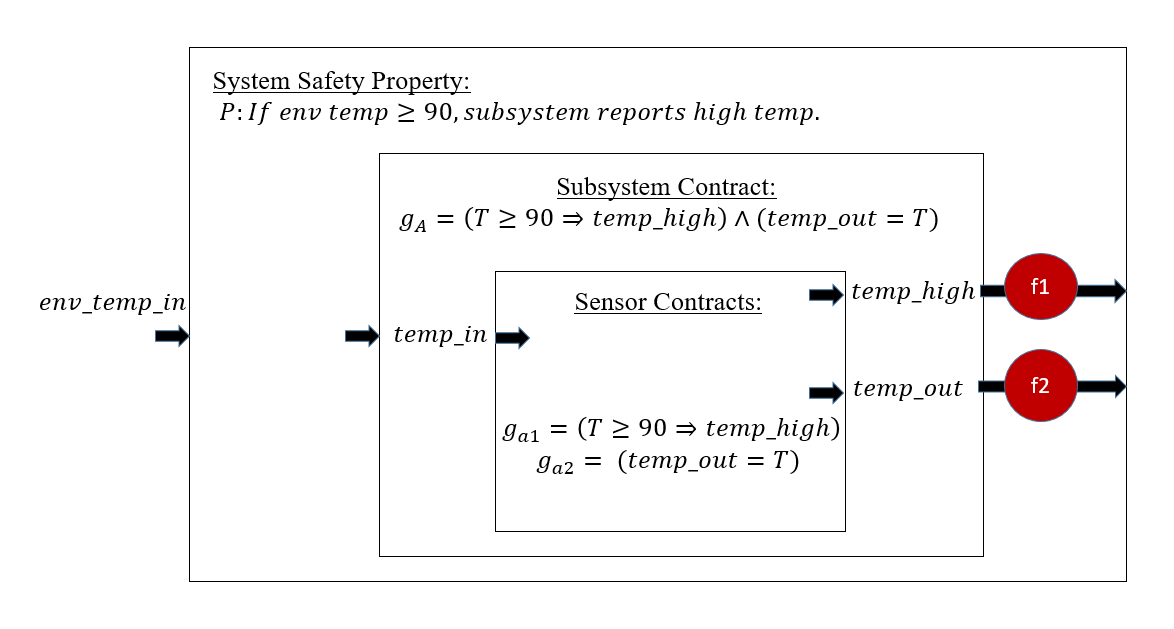
\includegraphics[width=10cm]{images/granularityEx.PNG}
\caption{Temp Sensor System Contract Part I} \label{fig:granularityEx1}
\end{center}
\end{figure}

The safety property at the top level requires the contract $g_A$ for proof of validity. Thus, the \aivcalg should contain the contract $g_A$ as an IVC. 

There are two faults defined for the temperature subsystem; one for each of the outputs. Fault $f_1$ affects the $temp\_high$ output and fault $f_2$ affects the $temp\_out$ output. Since each of these faults will violate the contract $g_A$, each of them should be found in the \textit{MinCutSet} for $G_A$.

Now assume that Figure~\ref{fig:granularityEx2} was the system contract representation built by engineer B. 

\begin{figure}[h!]
\begin{center}
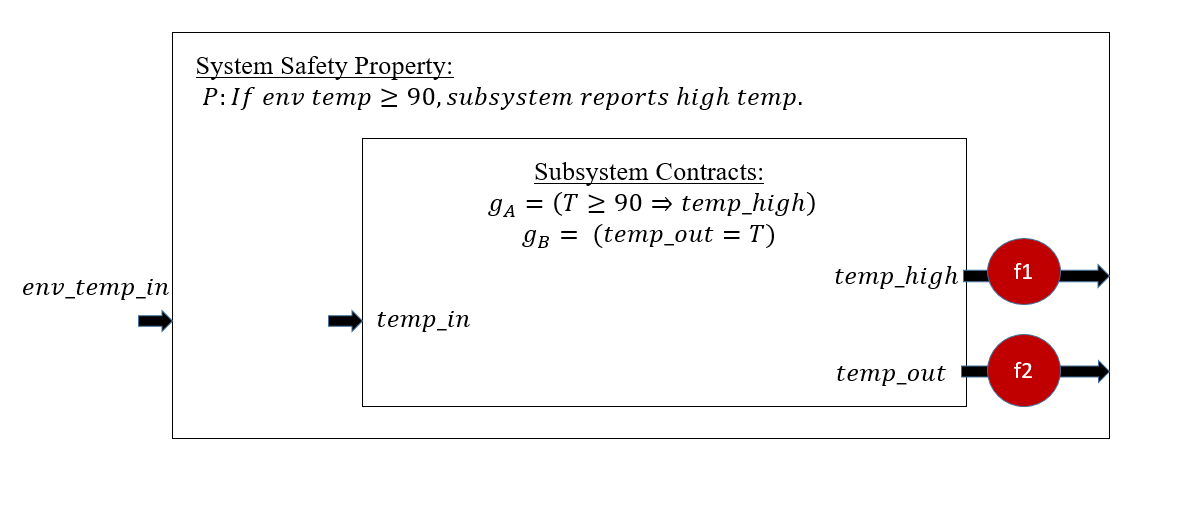
\includegraphics[width=10cm]{images/granularityEx2.PNG}
\caption{Temp Sensor System Contract Part II} \label{fig:granularityEx2}
\end{center}
\end{figure} 

The behavior and architecture of the system is the same, but the contract for the subsystem is more \textit{granular}; it is stated as two separate contracts:
\begin{center}
    $ g_A = (T \geq 90 \implies temp\_high)$ \\ 
    $ g_B = (temp\_indicator = T)$ 
\end{center}

Since $g_B$ is not required for the proof of the system safety property, only $g_A$ is found in the \textit{IVC}s and thus only $f_1$ will be seen in the \textit{MinCutSets} for this particular contract. 
 
In this simple example, it is easy to see how the granularity of the contracts may greatly affect the results of analysis.
\section{Algorithms and Results}
There were two main approaches that were taken to explore contractual granularity and how it may affect analysis results. The first approach was to automate contractual refinement and test results. The algorithms and descriptions of results can be found in Sections~\ref{sec:granularityANDAlg} and \ref{sec:granularityFRESHAlg}. The second approach included the use of {\em mutation} testing to find critical equations and contracts in the model, as well as critical node inputs. These results can be found in Sections~\ref{sec:granularityMutationEq} and \ref{sec:granularityMutationInputs}. 

All experimental results were run on a group of 15 AADL models annotated with AGREE contracts and fault models defined using the safety annex. The size of the models ranged from single layer with three instantiated components up to 5 layers with over 200 component instances. 

\subsection{Contractual Refinement}
The simplest restructuring that could be done on the model was to split any guarantees containing an $\land$ at the highest level of the binary Boolean statement and create additional guarantees from this split. For instance, if GUARANTEE0 = A and B, then split this into GUARANTEE1 = A, GUARANTEE2 = B. This provided an easy way to test that our assumption was correct regarding the types of minimal cut sets generated given various forms of contracts. Algorithm~\ref{alg:splitAnd} shows this process. 

\begin{algorithm}[h]
\SetKwFunction{FMain}{$splitOnAnd$}
 \SetKwProg{Fn}{Function}{:}{}

	\Fn{\FMain{expression}}{
		Program $P$ \;
		Guarantees $list_G$ \;
		\For{all $g \in list_G$}{
			\If{binary statement with operator $\land$}{
			    insert into $P$ $\rightarrow$ new guarantee (left) \;
			    insert into $P$ $\rightarrow$ new guarantee (right) \;
				splitOnAnd(left) \;
				splitOnAnd(right) \;
			} %end if there exists AND in G
		}%end for all g in P
	}
	\caption{Split guarantees on logical AND operator}
	\label{alg:splitAnd}
\end{algorithm}

The sensor encoded into Lustre originally has a single guarantee as shown in Figure~\ref{fig:lustreOneGuar} and the results of Algorithm~\ref{alg:splitAnd} can be seen in Figure~\ref{fig:lustreTwoGuar}. 

\begin{figure}[h!]
\begin{center}
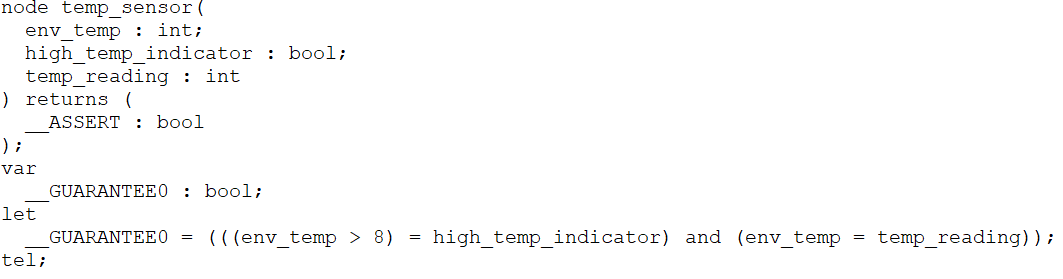
\includegraphics[width=1.0\textwidth]{images/lustreTwoGuar.PNG}
\caption{Temp Sensor With Original Guarantee} \label{fig:lustreOneGuar}
\end{center}
\end{figure} 

\begin{figure}[h!]
\begin{center}
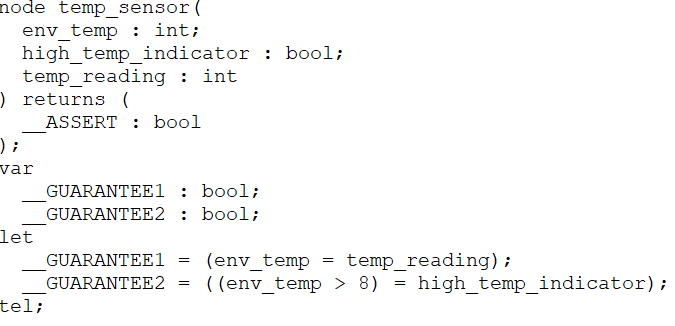
\includegraphics[width=.8\textwidth]{images/lustreOneGuar.PNG}
\caption{Temp Sensor With Modified Guarantees} \label{fig:lustreTwoGuar}
\end{center}
\end{figure} 

Given the property \texttt{((env\_temp $>$ 8) $=$ sensor\_high)}, in the first case, \texttt{GUARANTEE0} is the IVC. In the second case, only \texttt{GUARANTEE2} is the IVC for the property. The minimal cut sets produced reflected what we expected and show two faults in the cut set for Figure~\ref{fig:lustreOneGuar} and only the high temp indicator fault for the analysis in Figure~\ref{fig:lustreTwoGuar}. 

While this algorithm is efficient and quite simple, it only catches the low hanging fruit, so to speak. Due to the logical nature of how the Lustre model is analyzed, all guarantees are viewed as a conjunction; therefore, splitting guarantees into new statements only works on the $\land$ operator. This is sufficient for illustration and an initial test into the problem, but insufficient for full analysis of the issue. 

\danielle{Do some timing results to compare IVC generation and fault analysis with unmodified versions of projects. Put in results section?}
\subsection{Granular Refinement}
\label{sec:granularityFRESHAlg}
Model elements considered for the \aivcalg algorithm are explicitly defined in the Lustre code -- these we call \emph{IVC elements}; the generation of Lustre from an AADL/AGREE model provides guarantees and assumptions as IVC elements and when fault analysis is run using the safety annex, constrained faults are also added to this set. This can be seen in the safety analysis modified Lustre code in Figure~\ref{fig:lustreSensorsSafety} which is nominally the same as Figure~\ref{fig:lustreSensors}, but has faulty information added to outputs and IVC elements\footnote{For more information on safety modified Lustre programs, see Chapter XX, Section XX \danielle{ADD THIS TO IMPL}}. 

\danielle{Add figure of lustre code. Highlight IVC elements.}

\danielle{Wording in this paragraph.} We explored granularity within the context of the Lustre language; this programming language provides a nice formalism for discussion because it is top-level conjunctive, equational, and \emph{referentially transparent}: the behavior or a Lustre program is defined by a system of equations, and any subexpression on the right side of an equation can be extracted and assigned to a fresh variable which is substituted into the original equation without changing the meaning of a program~\cite{}(69). In this context, we can define a \emph{granular refinement} as an extraction of a subexpression into a new equation assigning a new variable. 

The maximal factorization of the model can be obtained by assigning each instance of a subexpression and each use of an input to its own variable. This results in a \emph{totally decomposed} Lustre model: (1) each computed (non-input) variable is used at most once in the right side of an equation, (2) each equation is either a single operator or a constant expression, and (3) each model input is directly assigned to one or more fresh variables and is not used elsewhere in the model~\cite{ghassabani_2018}.

Ghassabani did a preliminary analysis on maximally factored models for IVC coverage and found that analysis performed ``significantly slower" for proofs and the \ivcmust algorithm. For our purposes in safety analysis, our concern is both the faults and the guarantees in the Lustre model; therefore, we are able to weaken the factorization performed. In this research, a \emph{partially decomposed} Lustre model has the properties that (1) each computed variable is used at most once in the right side of a equation, and (2) each equation is either a single operator or a constant expression. 


\subsection{Mutations and Equation Removers}
\label{sec:granularityMutationEq}
For the development of model-based critical systems, it has been argued that formal proof should be applied to gain higher confidence in the model than with testing alone, e.g.~\cite{hardin2009development,miller2010software,rushby2009software,bozzano2003improving}. This has proven to be an active area of research, but has also shown some missing pieces -- one of which will be of benefit to us in this granularity exploration. When a property is proved valid, no further information is provided about the coverage of the model. One does not know whether the model contains features that are not covered by the properties~\cite{NFM2020Todorov}. Furthermore, we do not know if features \emph{within an IVC element in an MIVC set} are completely covered by the property. To this end, we began to look into mutation coverage to provide an answer. 

A mutation approach described by Todorov et al.~\cite{NFM2020Todorov} consists in mutating a model for which safety properties were proved valid, and trying to prove the same properties on the mutated models (\emph{mutants}). If the mutant is proved to be valid (i.e., it \emph{survived}), the mutant reveals part of the model that is not covered by the properties. We know that portion of the model is not necessary to find a proof. The approach described in this section attempts to use this type of mutant analysis on the contracts of a Lustre model, and thus compare to a granular refinement MIVC approach. 

A brief review of transition systems and some definitions are provided for convenience. 

Given a state space $U$, a transition system $(I,T)$ consists of an
initial state predicate $I : U \to \bool$ and a transition step
predicate $T : U \times U \to \bool$.
We define the notion of
reachability for $(I, T)$ as the smallest predicate $\reach : U \to
\bool$ which satisfies the following formulas:
\begin{gather*}
  \forall u.~ I(u) \Rightarrow \reach(u) \\
  \forall u, u'.~ \reach(u) \land T(u, u') \Rightarrow \reach(u')
\end{gather*}
A safety property $P : U \to \bool$ is a state predicate. A safety
property $P$ holds on a transition system $(I, T)$ if it holds on all
reachable states, i.e., $\forall u.~ \reach(u) \Rightarrow P(u)$,
written as $\reach \Rightarrow P$ for short. When this is the case, we
write $(I, T)\vdash P$.

The Lustre model is a set of equations$\{eq_1, \dots,eq_n\}$ and the transition relation $T$ has the structure of being a top level conjunction $T = t_1 \land \cdots \land t_n$ where each $t_i$ is an equality corresponding to $eq_i$. By further abuse of notation, $T$ is identified with the set of its top-level equalities. When an equation is removed from the Lustre model, an equality $t_i$ is removed from $T$ and the transition relation becomes $T\setminus \{t_i\}$. 

\begin{definition}
Minimal Inductive Validity Core (MIVC)~\cite{Ghassabani2017EfficientGO}: $S \subseteq T$ is a minimal Inductive Validity Core, denoted by $MIVC(P,S)$, iff $IVC(P,S) \land \forall T_i \in S$. $(I, S \setminus \{T_i\}) \not \vdash P$.
\end{definition}

In this research, we are only interested in minimal sets that satisfy a property $P$; if $(I, T) \vdash P$, then we know $P$ always has at least one MIVC which is not necessarily unique. By computing all MIVCs, we have a complete mapping from the requirements to the design elements; this is called \emph{complete traceability}~\cite{murugesan2016complete}. 

Ghassabani defines two metrics of coverage~\cite{ghassabani2017proof}. 

\begin{definition} \maycov\ : $t \in T$ is covered by $P$ iff $t_i \in $\maycov$(P)$, where \maycov$(P) = \{t_i | \exists S \in AIVC(P) \cdot t_i \in S\}$.
\end{definition}

\begin{definition} \mustcov\ : $t \in T$ is covered by $P$ iff $t_i \in $\maycov$(P)$, where \maycov$(P) = \{t_i | \forall S \in AIVC(P) \cdot t_i \in S\}$.
\end{definition}

The \maycov\ elements are relevant to the proof, but may be modified without affecting the satisfaction of $P$, whereas the \mustcov\ elements are absolutely necessary for the proof of $P$. One can view the \mustcov\ set of elements as the intersection of all MIVCs; if a single \mustcov\ element is removed, it ``breaks" all proofs of $P$. 

A mutator is formally a function that mutates any transition predicate $T$ to a set of mutants $\{T^1_{mut}, \dots, T^m_{mut}\}$, where each mutant $T^i_{mut}$ is obtained by applying a change to $T$. A very simple mutator is one that simply removes an equality $t_i$ from $T$, which amounts to removing the corresponding line of code from the Lustre model~\cite{NFM2020Todorov}. Todorov et al.~\cite{NFM2020Todorov} implemented an \emph{equation remover} in JKind which removes equations one by one and replays the proof process in an incremental way. If after removing an equation, the properties are still proved (the mutant survives), it means that the removed equation has no impact on the proof. If the properties do not hold any longer (the mutant is killed), then we know the removed equation is essential for the proof. This mutator computes the minimum \mustcov\ core. 


\subsection{Mutations and Guarantees}
\label{sec:granularityMutationInputs}
In the early stages of safety analysis on a complex critical system, it is beneficial to see what model elements may contribute to a property violation. While it is true that analysts will define faults based on their knowledge of the domain, at times in complex systems not all of these faults and their consequences are clear. Using the idea of mutations, we wish to see what the critical inputs to a system may be. 

As an example, we look once again at the sensor subsystem of a PWR as outlined in Chapter~\ref{chap:mcsGen}. Given a nominal system model containing the sensor subsystem and a single temperature sensor, we wish to see what model elements -- specifically guarantees -- are the \mustcov\  elements for the program. This tells the analyst that if these guarantees are violated, there are no paths to a proof of the property. 

To this end, we modified the equation remover implemented by Todorov, et al.~\cite{NFM2020Todorov} in JKind in order to collect killed guarantees from the program in Lustre. The analysis was run on a version of the sensor system with two subsystem guarantees: 

\begin{gather*}
\mathit{(env\_temp > 800) = high\_temp\_indicator}\\
\mathit{env\_temp = temp\_reading}
\end{gather*}

and one top level property:
\begin{gather*}
\mathit{(env\_temp > 800) = temp\_sensor\_high}\\
\end{gather*}

It is easy to see that a single subsystem level guarantee is sufficient to prove the property. The results from the modified equation remover shows the following guarantee that is critical to any proof of the safety property (Figure~\ref{fig:guaranteesKilledSensor}). The location referred to in the figure corresponds with the Lustre program line and column number for user reference.

\begin{figure}[h]
	\begin{center}
		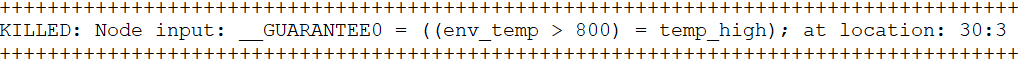
\includegraphics[scale=0.8]{images/guaranteesKilledSensor.PNG}
	\end{center}
	%\vspace{-1.5em}
	\caption{Temperature Subsystem Guarantee Killed by Equation Remover}
	\label{fig:guaranteesKilledSensor}
\end{figure}

After finding these results, we then defined a fault on the output governed by this guarantee and ran the minimal cut set generation on the fault model. As expected, this fault was in the minimal cut sets. While this example is sufficiently simple to illustrate the point, in complex models there can be multiple guarantees for a single component, many different components in a subsystem all of which are connected in various ways. It is obvious to anyone looking at the sensor subsystem model that this particular fault will violate the property. To this end, we turned our attention to a larger model: the Wheel Brake System as described in Section~\ref{chap:wbs}. At the time of this analysis, there were 33 fault nodes and 141 fault instances defined for 30 component types and 169 component instances throughout the extended system model. The total number of supporting guarantees within the nominal model was 246. We ran this analysis to see if there were other faults that may have been overlooked during the development of the WBS model. 

A guarantee on the hydraulic fuse component of the wheel brake subsystem was presented in a single layer mutation analysis as shown in Figure~\ref{fig:wheelBrakeGuaranteeKilled}. 

\begin{figure}[h]
	\begin{center}
		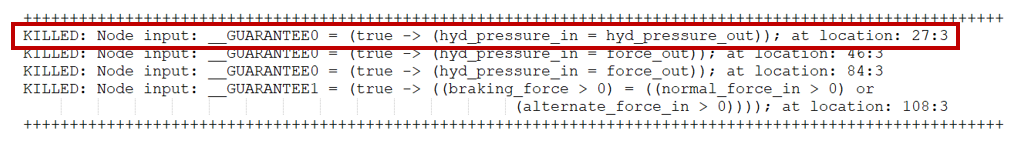
\includegraphics[scale=0.8]{images/wheelBrakeGuaranteesKilled.PNG}
	\end{center}
	%\vspace{-1.5em}
	\caption{Hydraulic Fuse Guarantee Killed by Equation Remover}
	\label{fig:wheelBrakeGuaranteeKilled}
\end{figure}

The guarantee presented governs the output of a hydraulic fuse attached to the wheel brake subsystem in the WBS. The guarantee states that the hydraulic pressure in is equal to the output. A stuck closed fault was defined on this fuse and minimal cut sets were generated for the WBS with cardinality restriction at one. Since this guarantee is a \mustcov\ element of the program, it should be the case that the fault is a single point of failure. The expected results are seen in the minimal cut sets as shown in Figure~\ref{fig:cutSetsWheelBrake}; the violation of the property occurs when this fault is present. 

\begin{figure}[h]
	\begin{center}
		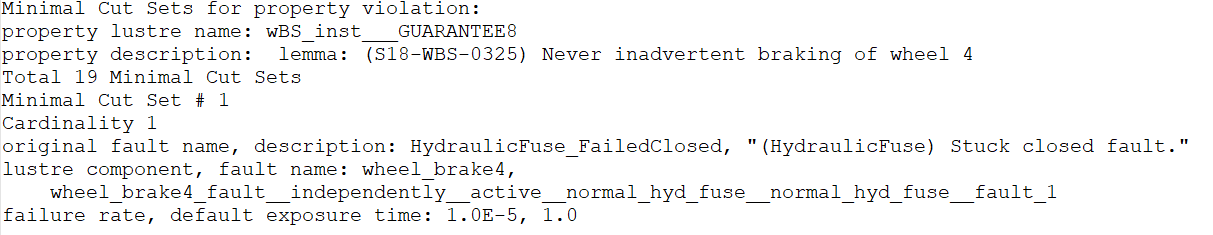
\includegraphics[scale=0.7]{images/cutSetsWheelBrake.PNG}
	\end{center}
	%\vspace{-1.5em}
	\caption{Hydraulic Fuse Fault in Minimal Cut Sets}
	\label{fig:cutSetsWheelBrake}
\end{figure}

Performing a kind of mutation analysis could be beneficial during the fault modeling process to catch things that may be missed during the fault definition process. The initial foray into mutation testing results show that this has potential for integration into the safety annex. It was also clear that a better presentation of the results was needed for large models. In the case of the WBS mutation analysis, over 240 guarantees were given as candidates for faults -- many of which already had faults associated with them. By integrating this feature into the fault analysis, these guarantees could be pruned from the output and save the user from pouring through potentially hundreds of guarantees as well as improve mutation engine time by eliminating the fault-associated guarantees from the analysis. Likewise, in the safety annex it is possible to generate the Lustre program if desired, but the common user will not reference the location of a guarantee this way. The location feature would need to be integrated into the safety annex and provide a link to the guarantee within the component AADL file.

\subsection{Node Inputs and Mutation Testing}
The equation remover mutation also iterates through Lustre node inputs and performs the mutation one input at a time. The node inputs in the Lustre model correspond to the inputs and outputs of an AADL component as shown in Figure~\ref{fig:nodeInputsLustre}. 

\begin{figure}[h]
	\begin{center}
		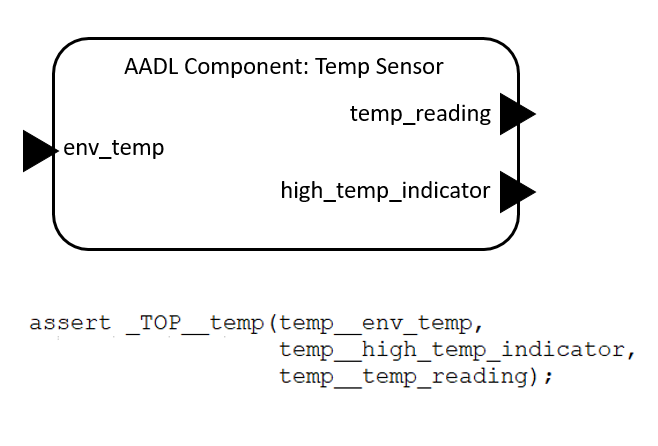
\includegraphics[scale=0.8]{images/nodeInputsLustre.PNG}
	\end{center}
	%\vspace{-1.5em}
	\caption{An AADL Component and Lustre Node Inputs}
	\label{fig:nodeInputsLustre}
\end{figure}

Given that the equation remover algorithm can perform this operation over node inputs, we can also gather information about critical outputs of components. Performing a similar extention to the equation remover algorithm, we collected all node input mutations that are killed and present them to the user. As an example, we show in Figure~\ref{fig:nodeInputsKilled} the analysis results on the nominal temperature subsystem example. 

\begin{figure}[h]
	\begin{center}
		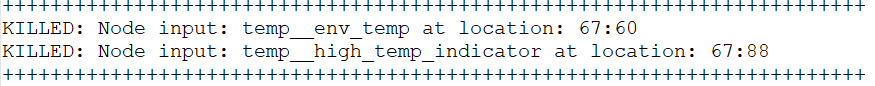
\includegraphics[scale=0.6]{images/nodeInputsKilled.PNG}
	\end{center}
	%\vspace{-1.5em}
	\caption{Temperature Node Inputs Killed by Equation Remover}
	\label{fig:nodeInputsKilled}
\end{figure}

Given that there exists an assumption on the temperature sensor input, we focus on the output. The only killed output was that of the high temperature indication, which tells us to prove the guarantee $\mathit{env\_temp} > 8 \iff \mathit{temp\_high}$, the output of this node is of utmost importance. Not surprisingly, when attaching a fault to this output, we get this fault in the minimal cut set for the top level property. 

As in the case with application of mutation testing on guarantees, node inputs also will require integration into the safety annex in order to filter out node inputs that have already been accounted for with faults in the extended system model. In large systems, this analysis is scalable and shows itself to be informative, but the outputs are unwieldy and large. Further work to rectify this would be required before use in large systems. 

The investigations into mutation testing applied to fault analysis were implemented in JKind and can be found at \url{https://github.com/dkstewart/jkind} on the {\em fault\_analysis\_mutations} branch.



\subsection{Discussion}